% Synchronized to r34917

\marklabel{chap:bootmedien}{
  \chapter{Creating the fli4l Archives/Boot media}
  }

  If all configuration is completed, the fli4l archives/boot media may be created
  as either bootable Compact-Flash, a bootable ISO image, or only the files needed
  for a remote update.

\marklabel{sec:bootmedien_linux}{
  \section{Creating the fli4l Archives/Boot media under Linux or other Unix derivatives and Mac OS X}
  }

  This is done by using scripts (\texttt{.sh}), which can be found in the
  fli4l root directory.

  \begin{description}
    \item \texttt{mkfli4l.sh}
  \end{description}

  The Build Script recognizes the different \jump{BOOTTYPE}{boot types}.

  The simplest call on Linux looks like this:
   \begin{verbatim}
    sh mkfli4l.sh
  \end{verbatim}

  The actions of the build scripts are controlled by three mechanisms:
   \begin{itemize}
    \item Configuration variable \var{BOOT\_TYPE} from
          \texttt{$<$config$>$/base.txt}
    \item Configuration file \texttt{$<$config$>$/mkfli4l.txt}
    \item Build-Script Parameters
  \end{itemize}

  The variable \jump{BOOTTYPE}{\var{BOOT\_TYPE}}
  decides which action of the Build Scripts is executed:
  \begin{itemize}
    \item Create a bootable fli4l CD-ISO-Image
    \item Generating the fli4l files needed for a remote update
    \item Generating the fli4l files and directly do a remote update via SCP
    \item a.s.o.
  \end{itemize}

  The description of the variables in the configuration file
  \texttt{$<$config$>$/mkfli4l.txt} can be found in Chapter
  \jump{sec:mkfli4lconf}{Control file mkfli4l.txt}.

  \subsection{Command line options}
  The last control mechanism is appending option parameters
  to the call of the Build Script on the command line.
  The control options correspond to those in the file \texttt{mkfli4l.txt}.
  Option parameters override the values from the control file.
  Out of convenience, the names of the option parameters differ from the names of
  the variables from the control file. There is a long and, to some extent, a
  short form:

  \begin{verbatim}
Usage: mkfli4l.sh [options] [config-dir]

-c, --clean         cleanup the build-directory
-b, --build <dir>   set build-directory to <dir> for the fli4l-files
-h, --help          display this usage
--batch             don't ask for user input

config-dir          set other config-directory - default is "config"

--hdinstallpath <dir> install a pre-install environment directly to
                    usb/compact flash device mounted or mountable to
                    directory <dir> in order to start the real installation
                    process directly from that device
                    device either has to be mounted and to be writable
                    for the user or it has to be mountable by the user
                    Do not use this for regular updates!

*** Remote-Update options
--remoteupdate        remote-update via scp, implies "--filesonly"
--remoteremount       make /boot writable before copying files and
                      read only afterwards
--remoteuser <name>   user name for remote-update - default is "fli4l"
--remotehost <host>   hostname or IP of remote machine - default
                      is HOSTNAME set in [config-dir]/base.txt
--remotepath <path>   pathname on remote maschine - default is "/boot"
--remoteport <portnr> portnumber of the sshd on remote maschine

*** Netboot options (only on Unix/Linux)
--tftpbootpath <path>   pathname to tftpboot directory
--tftpbootimage <name>  name of the generated bootimage file
--pxesubdir <path>      subdirectory for pxe files relative to tftpbootpath

*** Developer options
-u, --update-ver    set version to <fli4l_version>-rev<svn revision>
-v, --verbose       verbose - some debug-output
-k, --kernel-pkg    create a package containing all available kernel
                    modules and terminate afterwards.
                    set COMPLETE_KERNEL='yes' in config-directory/_kernel.txt
                    and run mkfli4l.sh again without -k to finish
    --filesonly     create only fli4l-files - do not create a boot-media
    --no-squeeze    don't compress shell scripts
    --rebuild       rebuild mkfli4l and related tools; needs make, gcc

    \end{verbatim}

   An HD pre-installation of a suitably formatted (FAT16/FAT32) CompactFlash
   (in a USB cardreader) or an USB Stick can be done by using the option
   \verb+--hdinstallpath <dir>+.
   You are using this script \emph{at your own risk}.
   The necessary fli4l files will be copied onto the specified partition.
   At first, run in the fli4l directory:

  \begin{verbatim}
     sh mkfli4l.sh --hdinstallpath <dir>
  \end{verbatim}
  \vspace{-2ex}
  This will generate the fli4l files and copy them to the CF-Card or USB Stick.

  To run the next steps, you have to make sure:

   \begin{itemize}
        \item \verb+chmod 777 /dev/brain+
        \item superuser rights
        \item installed \verb+syslinux+
        \item installed \verb+fdisk+
   \end{itemize}

 The script will ensure that this storage device is a FAT-partitioned USB-Drive.
 After that the boot loader and the files needed will be copied to the disk.
 You will get notified about success or failure.

 After the build you have to execute the following:

  \begin{verbatim}
    syslinux --mbr /dev/brain

    # make partition bootable using fdisk
    #     p - print partitions
    #     a - toggle bootable flag, specify number of fli4l partition
    #         usually '1'
    #     w - write changes and quit
    fdisk /dev/brain

    # install boot loader
    syslinux -i /dev/brain
 \end{verbatim}
 \vspace{-2ex}

 Now the CF resp. USB-drive should be bootable.
 Don't forget to unmount the device (via \texttt{umount}).

  \bigskip

  An alternative configuration directory can be specified by appending its name
  to the end of the command line. The normal configuration directory is called
  \texttt{config} and cn be found under the fli4l root directory. This is where all
  fli4l packages place their configuration files.
  If you want to maintain more than one configuration, create another directory, i.e. \texttt{hd.conf},
  place a copy of the configuration files there and change them according to the requirements.
  Here are some examples:

  \begin{verbatim}
     sh mkfli4l.sh --filesonly hd.conf
     sh mkfli4l.sh --no-squeeze config.test
  \end{verbatim}



\marklabel{sec:bootmedien_windows}{
  \section{Creating the fli4l Archives/Boot media under Windows}
  }

  Utilize the tool `AutoIt3' (\altlink{http://www.autoitscript.com/site/autoit/}). This enables a
  `graphical' edition, as well as dialogues which allow to change the variables described in the following
   sections.


  \begin{description}
    \item \texttt{mkfli4l.bat}
  \end{description}


  The Build program automatically recognizes the different \jump{BOOTTYPE}{boot types}.

  The `mkfli4l.bat' can be invoked directly from Windows Explorer, if you need no
  optional parameters.

   The actions of the Build program are controlled by different mechanisms:
  \begin{itemize}
    \item Configuration variable \var{BOOT\_TYPE} from the
          \texttt{$<$config$>$/base.txt}
    \item Configuration file \texttt{$<$config$>$/mkfli4l.txt}
    \item Parameter of the build program
    \item Interactive settings in the GUI
  \end{itemize}

  The variable \jump{BOOTTYPE}{\var{BOOT\_TYPE}} decides which action
  the Build program executes:
  \begin{itemize}
    \item Create a bootable fli4l CD-ISO-Image
    \item Making the fli4l files available, for remote update
    \item Generating the fli4l files and direct remote update via SCP
    \item Hard drive pre-install of a suitably formatted CF in the Cardreader
    \item a.s.o.
  \end{itemize}

  The description of the variables in the configuration file
  \texttt{$<$config$>$/mkfli4l.txt} can be found in Chapter
  \jump{sec:mkfli4lconf}{Control file mkfli4l.txt}.

  \subsection{Command line options}
  The last control mechanism is appending of option parameters to the call of the Build program
  on the command line. The control options correspond to those in the control file \texttt{mkfli4l.txt}. 
  Option parameters override the values from the control file.
  Out of convenience, the names of the option parameters differ from the names of
  the variables from the control file. There is a long and, to some extent, a
  short form:

  \begin{verbatim}
Usage: mkfli4l.bat [options] [config-dir]

-c, --clean             cleanup the build-directory
-b, --build <dir>       sets build-directory to <dir> for the fli4l-files
-v, --verbose           verbose - some debug-output
    --filesonly         creates only fli4l-files - does not create a disk
    --no-squeeze        don't compress shell scripts
-h, --help              display this usage

config-dir              sets other config-directory - default is "config"

*** Remote-Update options
--remoteupdate          remote-update via scp, implies "--filesonly"
--remoteuser <name>     user name for remote-update - default is "fli4l"
--remotehost <host>     hostname or IP of remote machine - default
                        is HOSTNAME set in [config-dir]/base.txt
--remotepath <path>     pathname on remote machine - default is "/boot"
--remoteport <portnr>   portnumber of the sshd on remote machine

*** GUI-Options
--nogui                 disable the config-GUI
--lang                  change language
                        [deutsch|english|espanol|french|magyar|nederlands]

  \end{verbatim}

  An alternative configuration directory can be passed by appending its name to the end of the command line.
  The normal configuration directory is called \texttt{config} and can be found under the fli4l
  root directory. This is where all fli4l packages place their configuration files.
  If you want to maintain more than one configuration, create another directory, e.g. \texttt{hd.conf},
  place a copy of the configuration files there and change it according to the requirements.
  Here are some examples:

  \begin{verbatim}
     mkfli4l.bat hd.conf
     mkfli4l.bat -v
     mkfli4l.bat --no-gui config.hd
  \end{verbatim}

  \subsection{Configuration dialog~-- Setting the configuration directory}

  In the main window the configuration directory setting is indicated and a window can be opened for
  the selection of the configuration directory.\\

  It should be noted that any change in the 'Config-Dir' causes all options to be set to the values contained in the
  \jump{sec: mkfli4lconf}{control file 'mkfli4l.txt'} placed in that directory, or to the values
  given as command-line parameters, respectively.\\

  If mkfli4l.bat does not find a directory fli4l-x.y.z$\backslash$config or if there is no file in that directory
  named `base.txt', a window is immediately opened for the selection of the configuration directory.
  This makes it possible to easily manage several fli4l configuration directories in a simple manner.\\

  Example:

\begin{example}
\begin{verbatim}
          fli4l-x.y.z\config
          fli4l-x.y.z\config.fd
          fli4l-x.y.z\config.cd
          fli4l-x.y.z\config.hd
          fli4l-x.y.z\config.hd-create
\end{verbatim}
\end{example}

  \subsection{Configuration dialog~-- General Preferences}
  \begin{figure}[ht!]
  \centering
  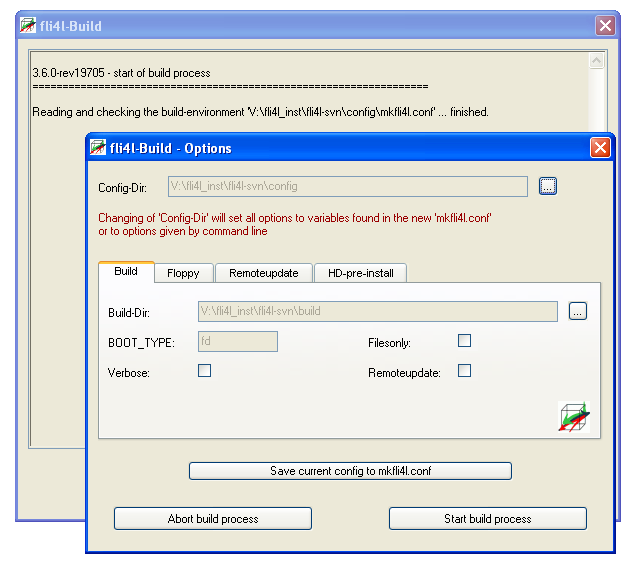
\includegraphics[width=\columnwidth]{win_build_build}
  \caption{Preferences}
  \label{fig:win_build_build}
  \end{figure}

  In this dialogue the settings are specified for the archive/boot-media
  creation:
  \begin{itemize}
    \item Build-Dir~-- Directory for the Archives/CD-Images/...
    \item \var{BOOT\_TYPE}~-- Display of the utilized/settings \var{BOOT\_TYPE}~-- unchangeable
    \item Verbose~-- Activation of additional output during the creation
    \item Filesonly~-- Only the archives are created~-- no bootmedia/no image
    \item Remoteupdate~-- Activation of the remote update via SCP
  \end{itemize}

  Using the button \textbf{Current settings in mkfli4l.txt buffer}
  the current settings can be stored in mkfli4l.txt.

  \subsection{Configuration dialog~-- Settings for Remote update}
  \begin{figure}[ht!]
  \centering
  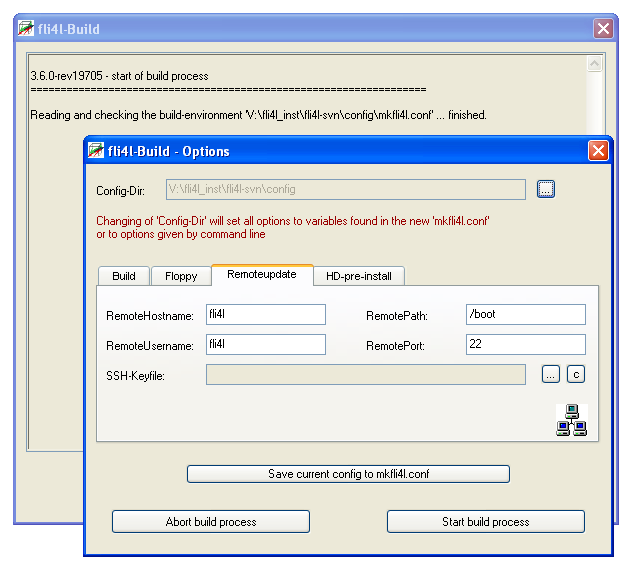
\includegraphics[width=\columnwidth]{win_build_remoteupdate}
  \caption{Settings for Remote update}
  \label{fig:win_build_remoteupdate}
  \end{figure}

  In this dialogue the settings for Remote update are specified:
  \begin{itemize}
    \item IP address or Hostname
    \item User name on the Remote host
    \item Remote path (default: /boot)
    \item Remote port (default: 22)
    \item SSH keyfile to use (format ppk from Putty)
  \end{itemize}

  \subsection{Configuration dialog~-- Settings for HD pre-install}
  \begin{figure}[ht!]
  \centering
  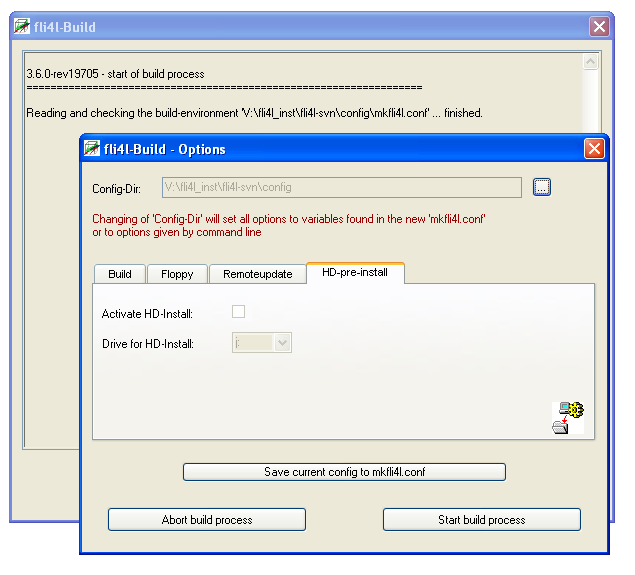
\includegraphics[width=\columnwidth]{win_build_hd_install}
  \caption{Settings for HD pre-install}
  \label{fig:win_build_hd_install}
  \end{figure}

   In this dialogue the options are set for HD pre-install on an
   accordingly partitioned and formatted Compact Flash card in a USB reader.

   Possible Options:
   \begin{itemize}
     \item Activate HD pre-install
     \item Drive letter to be used to access the CF card
  \end{itemize}

  Regarding the partitioning and formatting of the CF:
  A Type-A HD installation (see package HD) must be based on a primary, active,
  and formatted FAT partition on the CF card. If you would like to use a data partition
  additionally, a Linux partition which is formatted with the ext3 file system, as well as
  the file \texttt{hd.cfg} are also needed on the FAT Partiton (in this case please
  make sure to read the documentation of the HD package).

\marklabel{sec:mkfli4lconf}{
  \section{Control file mkfli4l.txt}}
  Since fli4l-Version 2.1.9 the control file
  \texttt{$<$config$>$/mkfli4l.txt} exists. This file can e.g. be used to specify
  directories which differ from the standard settings.
  The control file has a similar structure as the normal fli4l configuration files.
  All configuration variables here are optional, i.e. they need not exist or they can be commented out.
  \begin{description}

  \config {BUILDDIR}{BUILDDIR}{BUILDDIR}

  Default: `build'

  Specifies the directory where fli4l files will be created. If the variable is undefined,
  the Windows mkfli4l sets it to `build' relative to the fli4l root directory, resulting in
  the directory.
  \texttt{build} in the fli4l root directory:
  \begin{verbatim}
    Path/fli4l-x.y.z/build
  \end{verbatim}
  \vspace{-2ex}
  Under *nix mkfli4l is using \texttt{$<$config$>$/build} and is thus filing the
  generated files together with the configuration.

  The path for \var{BUILDDIR} must use the conventions of the Operating Systems
  Windows oder *nix. If relative paths configured there are converted by the build
  to the syntax of windows or *nix.

  \config {VERBOSE}{VERBOSE}{VERBOSE}

  Default: \var{VERBOSE='no'}

  Possible values are \var{'yes'} or \var{'no'}. Controls the \emph{Verbosity}
  of the Build Processes.

  \config {FILESONLY}{FILESONLY}{FILESONLY}

  Default: \var{FILESONLY='no'}

  Possible values are \var{'yes'} or \var{'no'}. This will actually
  turn off the creation of the boot-media and only the files will be created~--

  \config {REMOTEUPDATE}{REMOTEUPDATE}{REMOTEUPDATE}

  Default: \var{REMOTEUPDATE='no'}

  Possible values are \var{'yes'} or \var{'no'}. Enables automatic
  transferring of files by means of SCP to the router. This requires
  the package \jump{OPTSSHD}{SSHD} with activated \texttt{scp}.
  See also the following variables.

  \config {REMOTEHOSTNAME}{REMOTEHOSTNAME}{REMOTEHOSTNAME}

  Default: \var{REMOTEHOSTNAME=''}

  The target host name for the SCP data transfer.
  If no name is set, the variable
  \jump{HOSTNAME}{\var{HOSTNAME}} is used.

  \config {REMOTEUSERNAME}{REMOTEUSERNAME}{REMOTEUSERNAME}

  Default: \var{REMOTEUSERNAME='fli4l'}

  User name for the SCP data transfer.

  \config {REMOTEPATHNAME}{REMOTEPATHNAME}{REMOTEPATHNAME}

  Default: \var{REMOTEPATHNAME='/boot'}

  Destination path for the SCP data transfer.

  \config {REMOTEPORT}{REMOTEPORT}{REMOTEPORT}

  Default: \var{REMOTEPORT='22'}

  Destination port for the SCP data transfer.

  \config {SSHKEYFILE}{SSHKEYFILE}{SSHKEYFILE}

  Default: \var{SSHKEYFILE=''}

  Here you can specify a SSH key file for the SCP Remote update.
  Thus, an update can be made without specifying a password.

  \config {REMOTEREMOUNT}{REMOTEREMOUNT}{REMOTEREMOUNT}

  Default: \var{REMOTEREMOUNT='no'}

  Possible values are \var{'yes'} or \var{'no'}. If \var{'yes'}
  is set, a boot device "/boot" mounted read-only will be remounted
  read-write to allow remote updates of the boot files.

  \config {TFTPBOOTPATH}{TFTPBOOTPATH}{TFTPBOOTPATH}

  Path where the remote Netboot image is saved to.

  \config {TFTPBOOTIMAGE}{TFTPBOOTIMAGE}{TFTPBOOTIMAGE}

  Name of the Netboot image.

  \config {PXESUBDIR}{PXESUBDIR}{PXESUBDIR}

  Subdirectory for the PXE files relative to TFTPBOOTPATH.


  \config {SQUEEZE\_SCRIPTS}{SQUEEZE\_SCRIPTS}{SQUEEZESCRIPTS}

   Enable or disable the Squeezing (Compression) scripts.
   Compressing a script with Squeeze removes all comments and line indentations.
   Under normal conditions the default value of \var{'yes'} can be used.

  \config {MKFLI4L\_DEBUG\_OPTION}{MKFLI4L\_DEBUG\_OPTION}{MKFLI4LDEBUGOPTION}

   Additional debugging options can be handed over to the\jump{mkfli4l}{mkfli4l-Programm}.

  \end{description}

  \chapter{Connecting PCs in the LAN}

  For every host in the LAN you will have to set up:

  \begin{enumerate}
  \item IP address (see \smalljump{sec:pc-lan-ip}{IP address})
  \item Name of the host plus desired domain name
    (see \smalljump{sec:pc-lan-name}{Host and domain name})
  \item Default gateway (see \smalljump{sec:pc-lan-gateway}{Gateway})
  \item IP address of the DNS server (see \smalljump{sec:pc-lan-dns}{DNS server})
  \end{enumerate}

  \marklabel{sec:pc-lan-ip}{\section{IP address}}
  The IP address of the host has to belong to the same network as the IP
  address of the fli4l router (on the Ethernet interface), for example
  192.168.6.2 in case the router has the IP address 192.168.6.1.
  IP addresses have to be unique throughout the network, so it's a good idea to
  change (only) the last number. You will also have to make sure you specify
  the same IP address as specified in the file config/base.txt.

  \marklabel{sec:pc-lan-name}{\section{Host and domain name}}
  The name of the host is for example ``my-pc'', the domain ``lan.fli4l''.

  \wichtig{The domain set up on the host has to be identical to the domain
  set up on the fli4l if you want to use fli4l as a DNS server. Otherwise
  it could cause massive problems in the network.}

  The reason: Windows hosts regularly search for hosts within their
  workgroup, trying to resolve the name WORKGROUP.my-domain.fli4l. If the domain (here:
  my-domain.fli4l) doesn't match the one set up on the router, fli4l will try
  to answer the query by forwarding it to the Internet \ldots

  The domain has to be entered in the TCP/IP settings of the host.

  \subsection{Windows 2000}

  On Windows 2000 the settings can be found under:

  \noindent Start \pfeil\\
  \hspace*{2ex}Settings \pfeil\\
  \hspace*{4ex}Control Center \pfeil\\
  \hspace*{6ex}Network and Dial-up Connections \pfeil\\
  \hspace*{8ex}LAN Connection \pfeil\\
  \hspace*{10ex}Properties \pfeil\\
  \hspace*{12ex}Internet protocol (TCP/IP) \pfeil\\
  \hspace*{14ex}Properties \pfeil\\
  \hspace*{16ex}Extended\ldots \pfeil\\
  \hspace*{18ex}DNS \pfeil\\
  \hspace*{20ex}Add DNS-Suffix \pfeil\\

  Type ``lan.fli4l'' (or the domain set up~-- without ``''!)
  \pfeil Click OK.


\subsection{NT 4.0}

  Start \pfeil\\
  \hspace*{2ex}Settings \pfeil\\
  \hspace*{4ex}Control Center \pfeil\\
  \hspace*{6ex}Network \pfeil\\
  \hspace*{8ex}Protocols \pfeil\\
  \hspace*{10ex}TCP/IP \pfeil\\
  \hspace*{12ex}Properties \pfeil\\
  \hspace*{14ex}DNS \pfeil\\
  \hspace{16ex}\begin{itemize}
  \item Enter hostname (of the client)
  \item Enter domain (same as in config/base.txt)
  \item Add IP address of fli4l router
  \item Add DNS suffix (add domain~-- see two lines above)
  \end{itemize}

\subsection{Win95/98}

  Start \pfeil\\
  \hspace*{2ex}Settings \pfeil\\
  \hspace*{4ex}Control Center \pfeil\\
  \hspace*{6ex}Network \pfeil\\
  \hspace*{8ex}Configuration \pfeil\\
  \hspace*{10ex}TCP/IP (the one that is bound to the network\\
  \hspace*{10ex}interface to the router) \pfeil\\
  \hspace*{12ex}Properties \pfeil\\
  \hspace*{14ex}DNS Configuration:

  Activate DNS and under ``Domain:'' enter ``lan.fli4l'' (or the domain
  set up~-- without ``''!)

\subsection{Windows XP}

  On Windows XP the settings can be found at:

  \noindent Start \pfeil\\
  \hspace*{2ex}Settings \pfeil\\
  \hspace*{4ex}System Settings \pfeil\\
  \hspace*{6ex}Network Connections \pfeil\\
  \hspace*{8ex}LAN-Connection\pfeil\\
  \hspace*{10ex}Properties \pfeil\\
  \hspace*{12ex}Internetprotocol (TCP/IP) \pfeil\\
  \hspace*{14ex}Properties \pfeil\\
  \hspace*{16ex}Advanced\ldots \pfeil\\
  \hspace*{18ex}DNS \pfeil\\
  \hspace*{20ex}DNS-Suffix for this connection \pfeil\\

  Specify ``lan.fli4l'' (resp. the domain you use) (without ``''!)
  \pfeil Press OK.

\subsection{Windows 7}

  On Windows 7 the settings can be found at:

  \noindent Windows Button (ex. Start) \pfeil\\
  \hspace*{2ex}System settings \pfeil\\
  \hspace*{4ex}Network and Internet \pfeil\\
  \hspace*{6ex}Network- and Sharecenter \pfeil\\
  \hspace*{8ex}LAN-Connection\pfeil\\
  \hspace*{10ex}Properties \pfeil\\
  \hspace*{12ex}Internetprotocol Version 4 (TCP/IPv4) \pfeil\\
  \hspace*{14ex}Properties \pfeil\\
  \hspace*{16ex}Advanced \ldots \pfeil\\
  \hspace*{18ex}DNS \pfeil\\
  \hspace*{20ex}DNS-Suffix for this connection \pfeil\\

  Specify ``lan.fli4l'' (resp. the domain you use) (without ``''!)
  \pfeil Press OK.

\subsection{Windows 8}

  On Windows 8 the settings can be found at:

  \noindent Press Windows- and X-key simultaneously \pfeil\\
  \hspace*{2ex}System settings \pfeil\\
  \hspace*{4ex}Network and Internet \pfeil\\
  \hspace*{6ex}Network- and Sharecenter \pfeil\\
  \hspace*{8ex}Choose your net (Ehternet or WLAN) \pfeil\\
  \hspace*{10ex}Properties \pfeil\\
  \hspace*{12ex}Internetprotocol Version 4 (TCP/IPv4) \pfeil\\
  \hspace*{14ex}Properties \pfeil\\
  \hspace*{16ex}Advanced \ldots \pfeil\\
  \hspace*{18ex}DNS \pfeil\\
  \hspace*{20ex}DNS-Suffix for this connection \pfeil\\

  ``lan.fli4l'' (bzw. die eingestellte domain) eingeben (ohne ``''!)
  \pfeil OK drücken.
  \marklabel{sec:pc-lan-gateway}{\section{Gateway}}

  It is absolutely necessary to specify a default gateway, because without
  the correct IP address provided here nothing will work.
  So you will have to specify the IP address of the fli4l router here (the
  Ethernet interface's one)~-- for example 192.168.6.4, depending on the IP address
  that has been specified in the file config/base.txt for the router.

  It is wrong to enter fli4l as a proxy in the Windows or browser configuration
  unless you use a proxy on the router. Normally fli4l is not a proxy, thus
  please do \emph{not} specify fli4l as a proxy!

\marklabel{sec:pc-lan-dns}{\section{DNS server}}

  As for the IP address, you should not specify the IP address of the provider's
  DNS server, but the address of the router (Ethernet interface), as it
  will anwser queries itself or forward them to the Internet if needed.

  When fli4l is used as a DNS server, many queries from Windows hosts are not
  forwarded to the Internet but answered by fli4l itself.

\marklabel{sec:pc-lan-misc}{\section{Miscellaneous}}

  The items 1 to 4 do not have to be specified when a DHCP server is
  configured as fli4l transmits the needed data automatically.

  \textbf{Internet options:} Under connections you will have to select ``do not dial''.
  Under settings for local network (LAN): Do NOT enter anything (unless you use
  \var{OPT\_\-P}roxy). Both are default settings and should already exist.

\marklabel{IMONDSCHNITTSTELLE}{
  \chapter{Client/Server interface imond}
  }

  \marklabel{sec:imond}{
    \section{imon-Server imond}}

  imond is a network-capable server program that responds to certain queries
  or accepts commands that can control the router.

  imond also controls the Least-Cost-Routing. It uses the configuration
  file /etc/imond.conf, that is created automatically from the variables
  \var{ISDN\_\-CIRC\_\-x\_\-XXX} from the file config/isdn.txt and other
  at boot time by a shell script.

  imond runs permanentely as daemon and listens on TCP/IP port 5000 and the
  device /dev/isdninfo.


  All possible commands that can be sent to TCP/IP port 5000:
  \begin{table}
    \textbf{Admin commands}

    \vspace{1ex}
    \begin{tabular}{lp{9cm}}

      addlink ci-index              & Add channel to the circuit
                                      (channel bundling) \\
      adjust-time seconds           & Increments the date on the router by
                                      the number of seconds specified \\
      delete filename pw            & Deletes the file on the router \\
      hup-timeout \#ci-index [value]& Show or set the HUP timeout for
                                      ISDN circuits \\
      removelink ci-index           & Remove additional channel \\
      reset-telmond-log-file        & Deletes the telmond log file \\
      reset-imond-log-file          & Deletes the imond log file \\
      receive filename \#bytes pw   & Transfer a file to the router.
                                      Imond acknowledges the command using
                                      an ACK (0x06). After that, the file is
                                      transfered in blocks of 1024 bytes
                                      that are also acknowledged with an ACK.
                                      Finally, imond replies with an OK. \\
      send filename pw              & If the password is correct and the file
                                      exists, imond replies with OK \#bytes.
                                      Then, imond transfers the file in blocks
                                      of 1024 bytes that have to be
                                      acknowledged with an ACK (0x06).
                                      Finally, imond replies with an OK. \\
      support pw                    & Shows the status/configuration of the
                                      router \\
      sync                          & Syncs the cache of mounted drives \\
    \end{tabular}
  \end{table}

  \begin{table}
    \textbf{Admin or User commands}

    \vspace{1ex}
    \begin{tabular}{lp{9cm}}

      dial                      &    Dials the provider
                                     (Default-Route-Circuit) \\
      dialmode [auto|manual|off]&    Shows or sets the dialmode \\
      disable                   &    Hangs up and sets the dialmode to
                                     ``off'' \\
      enable                    &    Sets the dialmode to ``auto'' \\
      halt                      &    Cleanly shuts down the router \\
      hangup [\#channel-id]     &    Hangs up \\
      poweroff                  &    Shuts down the router and powers it off \\
      reboot                    &    Reboots the router \\
      route [ci-index]          &    Set the default route to circuit X
                                     (0=automatically) \\
    \end{tabular}
  \end{table}


  \begin{table}
    \textbf{User commands}

    \vspace{1ex}
    \begin{tabular}{lp{9cm}}
      channels                  & Shows the number of available ISDN
                                  channels\\
      charge \#channel-id       & Shows the online fee for a specific
                                  channel\\
      chargetime \#channel-id   & Time charged in consideration of the
                                  charge interval\\
      circuit [ci-index]        & Shows a circuit name\\
      circuits                  & Shows number of default-route-circuits\\
      cpu                       & Shows the CPU load in percent\\
      date                      & Shows date/time\\
      device ci-index           & Shows the device of the circuit\\
      driverid \#channel-id     & Shows driver-id of the channel X\\
      help                      & Shows help\\
      inout \#channel-id        & Shows direction (incoming/outgoing)\\
      imond-log-file            & Shows imond log file\\
      ip \#channel-id           & Shows IP\\
      is-allowed command        & Shows, whether a command is
                                  configured/allowed\newline
                                  Possible commands:
                                    dial|dialmode|route|reboot|
                                    imond-log|telmond-log|mgetty-log \\
      is-enabled                & Shows, whether dialmode is off (0) or auto
                                  (1)\\
      links ci-index            & Show number of channels 0, 1 or
                                  2, 0 means: No channel bundling possible\\
      log-dir imond|telmond|mgetty& Shows the log directory\\
      mgetty-log-file           & Shows mgetty logfile\\
      online-time \#channel-id  & Shows online time of the current connection
                                  in hh:mm:ss\\
      pass [password]           & Show, whether it is necessary to enter a
                                  password or enter a password\newline
                                  1 Userpassword is set\newline
                                  2 Adminpassword is set\newline
                                  4 imond is in admin mode\\
      phone \#channel-id        & Show telephone number/name of the peer\\
      pppoe                     & Show the number of pppoe devices (i.e. 0
                                  or 1)\\
      quantity \#channel-id     & Show the data transferred in bytes\\
      quit                      & Terminates the connection to imond\\
      rate \#channel-id         & Show transfer rates (incoming/outgoing
                                  in B/sec)\\
      status \#channel-id       & Show status of channel X\\
      telmond-log-file          & Shows telmond log files\\
      time \#channel-id         & Show the sum of online times, format
                                  hh:mm:ss\\
      timetable [ci-index]      & Shows the time table for the LC-Routing\\
      uptime                    & Shows the uptime of the router in seconds\\
      usage \#channel-id        & Show the type of connection, that is available
                                  responses: Fax, Voice, Net, Modem, Raw\\
      version                   & Show the protocol and program version\\
    \end{tabular}
  \end{table}

The TCP/IP port 5000 is only reachable from the masqueraded LAN.
  Access from remote is blocked by the firewall configuration by default.

  Imond supports two user levels: the user and the admin mode. For both
  levels you can set a password using var{IMOND\_\-PASS} and/or
  \var{IMOND\_ADMIN\_\-PASS}. Then, clients are forced by imond to
  submit a password. As long as no password has been submitted, only the
  commands ``pass'' and``quit'' are accepted. Others are rejected.

  If you want to further restrict access, e.g. only allow access
  from a single computer, the firewall configuration has to be changed.

  At present this is not possible using the standard configuration files
  config/base.txt. You will have to change the file /etc/rc.d/rc322.masq.

  The commands

\begin{example}
\begin{verbatim}
         enable/disable/dialmode   dial/hangup   route   reboot/halt
\end{verbatim}
\end{example}

  Can be globally enabled/disabled using the configuration variables
  \var{IMOND\_\-XXX} (see ``Configuration'').

  From a Unix/Linux computer (or a Windows computer in a DOS box) you can
  easily try it out:
  Type

\begin{example}
\begin{verbatim}
        telnet fli4l 5000        \# or the appropriate name of the fli4l-Routers
\end{verbatim}
\end{example}

  and you will be able to directly enter the listed commands and look at
  the output.

  For example after entering ``help'' the help is shown, after
  ``quit'' the connection to imond is terminated.

\marklabel{sec:leastcostrouting}{
  \subsection{Least-Cost-Routing~-- how it works}
  }

  imond contructs a table (time table) from the configuration file
  /etc/imond.conf (which is created on bootup from the config variables
  \var{ISDN\_\-CIRC\_\-x\_\-TIMES} and others). It contains a complete
  calendar week in a raster of 1 hour (168 hours = 168 Bytes). But the
  table only contains the circuits that have a default route defined.

  Using the imond command ``timetable'' you can have a look at it.

  Here an example:

  Supposing 3 circuits are defined:

\begin{example}
\begin{verbatim}
        CIRCUIT_1_NAME='Addcom'
        CIRCUIT_2_NAME='AOL'
        CIRCUIT_3_NAME='Firma'
\end{verbatim}
\end{example}

   Only the first two circuits have a default circuit defined, i.e. the
  corresponding variables ISDN\_CIRC\_x\_ROUTE have the value '0.0.0.0'.

  If the variables \var{ISDN\_\-CIRC\_\-x\_\-TIMES} look like this:

\begin{example}
\begin{verbatim}
        ISDN_CIRC_1_TIMES='Mo-Fr:09-18:0.0388:N Mo-Fr:18-09:0.0248:Y
                      Sa-Su:00-24:0.0248:Y'

        ISDN_CIRC_2_TIMES='Mo-Fr:09-18:0.019:Y Mo-Fr:18-09:0.049:N
                      Sa-Su:09-18:0.019:N Sa-Su:18-09:0.049:N'

        ISDN_CIRC_3_TIMES='Mo-Fr:09-18:0.08:N Mo-Fr:18-09:0.03:N
                      Sa-Su:00-24:0.03:N'
\end{verbatim}
\end{example}

  it results in the following /etc/imond.conf being created:

\begin{example}
\begin{verbatim}
        #day  hour  device  defroute  phone        name        charge  ch-int
        Mo-Fr 09-18 ippp0   no        010280192306 Addcom      0.0388   60
        Mo-Fr 18-09 ippp0   yes       010280192306 Addcom      0.0248   60
        Sa-Su 00-24 ippp0   yes       010280192306 Addcom      0.0248   60
        Mo-Fr 09-18 ippp1   yes       019160       AOL  0.019   180
        Mo-Fr 18-09 ippp1   no        019160       AOL  0.049   180
        Sa-Su 09-18 ippp1   no        019160       AOL  0.019   180
        Sa-Su 18-09 ippp1   no        019160       AOL  0.049   180
        Mo-Fr 09-18 isdn2   no        0221xxxxxxx  Firma       0.08     90
        Mo-Fr 18-09 isdn2   no        0221xxxxxxx  Firma       0.03     90
        Sa-Su 00-24 isdn2   no        0221xxxxxxx  Firma       0.03     90
\end{verbatim}
\end{example}

  imond creates the following time table in memory~-- here the output
  of the imond command ``timetable'':

\begin{example}
\begin{verbatim}
         0  1  2  3  4  5  6  7  8  9 10 11 12 13 14 15 16 17 18 19 20 21 22 23
     --------------------------------------------------------------------------
     Su  3  3  3  3  3  3  3  3  3  3  3  3  3  3  3  3  3  3  3  3  3  3  3  3
     Mo  2  2  2  2  2  2  2  2  2  4  4  4  4  4  4  4  4  4  2  2  2  2  2  2
     Tu  2  2  2  2  2  2  2  2  2  4  4  4  4  4  4  4  4  4  2  2  2  2  2  2
     We  2  2  2  2  2  2  2  2  2  4  4  4  4  4  4  4  4  4  2  2  2  2  2  2
     Th  2  2  2  2  2  2  2  2  2  4  4  4  4  4  4  4  4  4  2  2  2  2  2  2
     Fr  2  2  2  2  2  2  2  2  2  4  4  4  4  4  4  4  4  4  2  2  2  2  2  2
     Sa  3  3  3  3  3  3  3  3  3  3  3  3  3  3  3  3  3  3  3  3  3  3  3  3

     No.  Name                   DefRoute  Device  Ch/Min   ChInt
      1   Addcom                   no      ippp0   0.0388     60
      2   Addcom                   yes     ippp0   0.0248     60
      3   Addcom                   yes     ippp0   0.0248     60
      4   AOL               yes     ippp1   0.0190    180
      5   AOL               no      ippp1   0.0490    180
      6   AOL               no      ippp1   0.0190    180
      7   AOL               no      ippp1   0.0490    180
      8   Firma                    no      isdn2   0.0800     90
      9   Firma                    no      isdn2   0.0300     90
     10   Firma                    no      isdn2   0.0300     90
\end{verbatim}
\end{example}

  For circuit 1 (Addcom) there are three time ranges (1-3) defined.
  For circuit 2 (AOL) there are four time ranges (4-7) and
  for the last one there are three time ranges (8-10).

  In the time table, the indices are printed that are valid in the
  corresponding hour. Only the indices 2-4 show up here, as the others
  are not default routes.

  If there are zeros in the table, there are gaps in the values of the
  \var{ISDN\_\-CIRC\_\-X\_\-TIMES} variables. At this point there is no
  default route, no internet access is possible!

  On program start, imond checks for the weekday and the hour. Then, the
  index from the time table is picked out and the corresponding circuit.
  The default route is then set to this circuit.

  If the status of a channel changes (e.g. offline~-- online) or at least
  after one minute, this procedure is repeated: check time, lookup
  in table, pick default route circuit.

  If the used circuit changes, e.g. on mondays, 18:00, the default route
  is deleted, existing connections are terminated (sorry\ldots) and after
  that the default route is set to the new circuit. Imond may notice this
  up to 60 seconds too late~-- so at least at 18:00:59 the route is
  changed.

  If a circuit does not have a default route, nothing will change. The value
  of \var{ISDN\_\-CIRC\_\-x\_\-TIMES} is only used to calculate the fee.
  This can be important if the LC routing is disabled temporarily, e.g. using
  the client imonc, and a circuit is dialed manually.

  But you can have a look at the tables for other time-range-indices
  (in our example 1 to 10), also at the ones of the
  ``Non-LC-Default-Route-Circuits''.

  Command:

\begin{example}
\begin{verbatim}
                    timetable index
\end{verbatim}
\end{example}

  Example:

\begin{example}
\begin{verbatim}
                    telnet fli4l 5000
                    timetable 5
                    quit
\end{verbatim}
\end{example}

  The output will look like:

\begin{example}
\begin{verbatim}
         0  1  2  3  4  5  6  7  8  9 10 11 12 13 14 15 16 17 18 19 20 21 22 23
     --------------------------------------------------------------------------
     Su  0  0  0  0  0  0  0  0  0  0  0  0  0  0  0  0  0  0  0  0  0  0  0  0
     Mo  5  5  5  5  5  5  5  5  5  0  0  0  0  0  0  0  0  0  5  5  5  5  5  5
     Tu  5  5  5  5  5  5  5  5  5  0  0  0  0  0  0  0  0  0  5  5  5  5  5  5
     We  5  5  5  5  5  5  5  5  5  0  0  0  0  0  0  0  0  0  5  5  5  5  5  5
     Th  5  5  5  5  5  5  5  5  5  0  0  0  0  0  0  0  0  0  5  5  5  5  5  5
     Fr  5  5  5  5  5  5  5  5  5  0  0  0  0  0  0  0  0  0  5  5  5  5  5  5
     Sa  0  0  0  0  0  0  0  0  0  0  0  0  0  0  0  0  0  0  0  0  0  0  0  0

     No.  Name                   DefRoute  Device  Ch/Min   ChInt
      5   AOL               no      ippp1   0.0490    180
\end{verbatim}
\end{example}

  Got everything?

  Using the command ``route'', the LC routing can be enabled or disabled.
  If a positive circuit index is specified (1\ldots N) the default route
  is changed to the circuit specified. If the index is 0, LC routing will be
  activated again and the active circuit is chosen automatically.


  \subsection{Annotations to the calculation of the online changes}

  The whole model how the online charges are calculated will only work
  correctly, if the charge interval for a single circuit (variable
  \var{ISDN\_\-CIRC\_\-x\_\-CHARGEINT}) remains constant throughout the whole
  week.

  Normally, this is correct for most of the internet providers. But if you
  dial in, e.g. to your companies network, using the (German) Telecom (not
  the internet provider T-Online), the change interval changes at 18:00 from
  90 seconds to 4 minutes (information from June 2000). Because of that, the
  definition

\begin{example}
\begin{verbatim}
        ISDN_CIRC_3_CHARGEINT='90'
        ISDN_CIRC_3_TIMES='Mo-Fr:09-18:0.08:N Mo-Fr:18-09:0.03:N Sa-Su:00-24:0.03:N'
\end{verbatim}
\end{example}

  is not absolutely correct. After 18:00 the price is converted to 3
  cents (4 minutes cost 12 cents), but the charge interval is wrong.
  Because of that, the displayed charge could differ from the actual one.

  Here is a tip, how different charge intervals can be handled correctly,
  anyhow (also important for \var{ISDN\_\-CIRC\_\-x\_\-CHARGEINT}):
  Just define 2 cicuits~-- one for each charge interval.
  Of course you will have to adjust \var{ISDN\_\-CIRC\_\-x\_\-TIMES}
  so that the valid circuit is always dialed, depending on the charge
  interval.

  Once again: If you connect to an ISP you most likely will not have this
  problem, because the charge interval is constant all the time and
  only the prices per minute change (or doesn't it? I guess the German
  provider T-* could even introduce such a price model :-).

  % Synchronized to r30003
  \marklabel{sec:winimonc}{
    \section{Windows-Client imonc.exe}}

  \subsection{Introduction}

  imond on the router and on the client imonc as a team have
  two use modes: the user and the admin mode. In admin mode, all
  controls are enabled. In user mode the variables
  \jump{IMONDENABLE}{\var{IMOND\_ENABLE}}, \jump{IMONDDIAL}{\var{IMOND\_DIAL}}, 
  \jump{IMONDROUTE}{\var{IMOND\_ROUTE}} and \jump{IMONDREBOOT}{\var{IMOND\_REBOOT}}
  control if the respective functions are available. If all of these
  variables are set to `no ', this means that all buttons in the overview page
  are disabled except for the exit and the admin mode button. The
  decision whether the user or admin mode is used, is based on the
  transmitted password. By clicking the button admin mode, located in the
  status bar, you may switch to the admin mode at any time by entering the
  admin password. To switch back imonc must be restarted.

  Once imonc is started an additional tray icon is displayed, which
  shows the connection status of existing channels.

  The colors mean:
  \begin{description}
    \item[Red]: Offline
    \item[Yellow]: A connection is in the process of being established
    \item[Light Green]: Online and traffic on the channel
    \item[Dark Green]: Online and (nearly) no traffic on the channel
  \end{description}

  \noindent imonc shows a behavior a little different from the Windows standard
  when clicking on the minimize button in the title bar. This minimizes imonc
  to the system tray only a tray icon near the clock remains. Double clicking
  on the tray icon with the left mouse button brings imonc's window back to
  the foreground. With the right mouse button you may use the context menu,
  of the tray icon to execute the main imonc commands die angezeigten
         without displaying its
  main window.

  Imonc stores many properties (including all columns widths of the string grids)
  in the registry, so its appearance may be widely adapted to your needs. Imonc
  uses the registry key HKCU{\textbackslash}Software{\textbackslash}fli4l
  to store this informations

  If even after careful reading of the documentation problems on imonc or the
  router itself still remain you can post to the newsgroup. It makes sense
  to note the support information you get when choosing SystemInfo and then Info
  on the About page of the imonc client. The router password will be queried
  then (not the imond password) and after that imonc will create a file fli4lsup.txt
  that contains all the important information regarding the router, including
  imonc. This file can be posted on the newsgroup when explicitely demanded
  and will give much better chance for quick help.

  Further details concerning the development of the Windows imonc client can be found
  on the homepage of Windows Imonc \altlink{http://www.imonc.de/}. Here you can
  see what new features and bug fixes will be included in the next version.
  In addition, you will find the latest imonc version, if it is not included
  in the FLI4L distribution already.

  \subsection{Start Parameters}

  Imonc requires the name or IP address of the router fli4l. As the default
  the program attempts to establish a connection with the computer ``fli4l''.
  If this entry is correctly entered in the DNS, this should work out of the box.
  Otherwise you can pass following parameters in the link:

  \begin{itemize}
    \item /Server:The router's IP or hostname (short form: /S:IP or hostname)
    \item /Password:password (short form: /P:password)
    \item /log Option for logging communication betweeen imonc und imond. When
      entered a file imonc.log  will be written each time when imonc exits. It
      contains the complete communication and thus can grow quite large. Please
      use this parameter only in case of problems.
    \item /iport:Portnumber Portnumber imond listens to. Default: 5000
    \item /tport:Portnummer Portnumber telmond listens to. Default: 5001
    \item /rc:''Command'' The command provided here will be transmitted to the
      router without further checking and imonc will exit afterwards. 
      If more than one command should be transmitted at once, they must be devided
      by semicolons. You will have to provide an imond password in addition for
      this to work because no password query will be queried. Possible command
      are documented with imond, see chapter 8.1. In addition to the commands
      there another one exists: timesync. If used imonc will synchronize the
      clock of the client with the router's clock. The command dialtimesync is
      not supported anymore, it is substituted by "dial; timesync".
    \item /d:''fli4l-Directory'' Pass the fli4l-directory as a start parameter.
      May be of interest when using more than one fli4l version.
    \item /wait If the hostname can't be reolved imonc will not exit anymore~--
      start another try by doubleclicking the tray icon.
    \item /nostartcheck Disables checking of imonc already running. Only makes
      sense to monitor several different fli4l routers in a net. When using more
      instances the builtin syslog- and \mbox{E-Mail}-capabilites will be disabled.
  \end{itemize}

  Usage (to be entered in the link):

\begin{example}
\begin{verbatim}
X:\...imonc.exe [/Server:Host] [/Password:Password] [/iport:Portnumber]
            [/log] [/tport:Portnumber] [/rc:"Command"]
\end{verbatim}
\end{example}

  Example with IP address:

\begin{example}
\begin{verbatim}
        C:\wintools\imonc /Server:192.168.6.4
\end{verbatim}
\end{example}

  or with name and password:

\begin{example}
\begin{verbatim}
        C:\wintools\imonc /S:fli4l /P:secret
\end{verbatim}
\end{example}

  or with name and password and router command:

\begin{example}
\begin{verbatim}
        C:\wintools\imonc /S:fli4l /P:secret /rc:"dialmode manual"
\end{verbatim}
\end{example}

  \subsection{Overview}

  The Windows client queries some imond information on the existing
  connections and displays it in its window. In addition to general
  status information such as uptime of the router or the time (both locally
  and on the router), for each existing connection the following informations
  are shown:

  \begin{tabular}{lp{9cm}}
    Status             &Connection establishment/Online/Offline\\
    Name               &Telephone number of the caller or circuit name\\
    Direction          &Indicates if a connection is incoming or outgoing\\
    IP                 &IP, that was assigned to the router\\
    IBytes             &Bytes received\\
    OBytes             &Bytes sent\\
    Online time        &Actual online time\\
    Time               &Sum of all online times\\
    KTime              &Sum of all online times in consideration of charge intervals\\
    Cost               &Computed costs\\
  \end{tabular}

  \medskip

  The data is updated every 2 seconds by default. In the context menu of
  this overview it is possible to copy the assigned IP to the clipboard
  as well as hanging up the channel (for each available channel which is
  online at the moment). This is of interest in case that several different
  connections exist, e.g. one to surf the Internet and another to a private
  net and only one of them should be terminated.

  If the telmond process is active on the router, imonc can show information
  about incoming phone calls (ie calling and called MSN) in addition. The last
  incoming phone call is displayed above the buttons. a log of phone calls received
  can be obtained by viewing the calls page.

  By the six buttons in imonc the following commands can be selected:

  \begin{tabular}{clp{9cm}}
    Button & Caption & Function \\
    1& Connect/Disconnect &   Dial/Hang up\\
    2& Add link/Rem link  &   Bundle channels: yes/no~-- only available in admin mode\\
    3& Reboot             &   Reboot fli4l!\\
    4& PowerOff           & Shut down fli4l and power off afterwards\\
    5& Halt               & Shut down fli4l to power off safe afterwards\\
    6& Exit               & Exit client\\
  \end{tabular}

  \medskip

  \noindent The first five commands can be switched on and off individually in the
  router's configuration file config/base.txt for the user mode. In admin mode all
  are enabled. The dialmode controls the dialing behavior of the router:

  \begin{tabular}{lp{9cm}}
    Auto  & The router will establish connections automatically when getting 
    queries from the local net for the circuit concerned.\\
    Manual & The user himself has to establish connections.\\
    Off   & No connections can be established. The dial button is deactivated.\\
  \end{tabular}

  \medskip

  \noindent Note that fli4l by default will dial out independently. So you never
  actually will have to press the connect button\ldots

  It is also possible to manually switch the default route circuit, setting
  the automatic LCR on and off. In the Windows version of imonc the selection
  list `` default route'' is provided for this. In addition you can configure the
  hangup TimeOut time directly in imonc. use the Config button next to the default
  route for this. All configured circuits of the router are displayed here. The
  value in the column Hup-timeout can be edited directly in the string grid
  for ISDN circuits (not yet working for DSL).

  An overview over LCR can be found on the page admin/Timetable.
  There you'll see what circuit imond selects automatically at which time.

  \subsection{Config-Dialog}

  The configuration is reached using the Config button in the status bar. The window
  is divided into the following areas:

  \begin{itemize}
  \item The Area General:
    \begin{itemize}
    \item Actualization Interval: Set here how often the overview should get actualized.
    \item Synchronize Time on Startup: When starting the client's system time and date 
      will get synchronized with the router's system time. You can execute this manually
      by using the button Synchronize on the Overview-page.
    \item Start Minimized: Program will start minimized to the system tray.
    \item Start with Windows: Specify here if the client should start automatically 
      with system start. Provide necessary start-parameters in the field Parameter.
    \item Fetch News from fli4l.de: Should news from fli4l's homepage be fetched and
      displayed by imonc? Then headlines are shown in the status bar. A new page News
      is displayed to show the complete messages.
    \item Logfile for Connections: The file name here is used to save connection lists
      locally on the imonc's system.
    \item TimeOut for router to answer: How long should we wait for an answer from the
      router before assuming that the connection has failed.
    \item Language: Pick the language for imoncs to use.
    \item Confirm Router Commands: If activated all commands influencing the router
      generally have to be confirmed, i.e. Reboot, Hangup \ldots
    \item Hang up even when traffic: No information should be displayed when the
      connection is closed and there is still traffic on the line.
    \item Automatic Connection to the router: Should we try to reconnect to the router
      in case of lost connections (i.e. when rebooting the router).
    \item Minimize Window To System Tray: Should imonc minimize to system tray instead
      of terminating itself when clicking the Exit button.
    \end{itemize}

  \item Proxy Settings:
    Define a proxy for imonc's http-queries here. It will be used for fetching news.
    \begin{itemize}
    \item Activate Proxy-support for Http-queries: Should we use a proxy 
          \begin{itemize}
            \item Address: Address of the proxy server
            \item Port: Port number of the proxy server (default: 8080)
          \end{itemize}
    \end{itemize}
    
  \item TrayIcon:
  	Set the colors of the tray icon next to the clock to your own needs.
  	In addition you can specify that the actual dialmode will set the background
  	color of the tray icon.

  \item Calls: The position of the call notification window will be saved in the
    registry in order to allow to set a fixed position for the window. Simlpy drag the
    window to the desired position.
    \begin{itemize}
      \item Update: Set here in what way imonc will be informed about new calls. There
	are three possibilities. The first is querying the telmond service on the
	router in regular time intervals. A second is evaluating the syslog messages.
	This variant is preferred to the first~- of course, the imon's syslog client
	has to be enabled. If imonc is used with a routed eisfair system the third
	possibility is to use the Capi2Text package for call signaling.
      \item Delete Leading Zeros (Phone Boxes): Phone boxes often use an additional
	Zero to prefix the caller's number. This option will suppress the digit.
      \item Own Area Code: Save your own area code here. If a call with the same
	area code is received it will get suppressed when displaying.
      \item Telephone Book: Here, the file can be specified, in which the local
        Phone book is saved for resolving of the phone number. If the file does not
        exist, it is created by the program.
      \item Logfile: The file name you can specify here is used to save the call
	list locally on the computer. This menu item is only visible if the config
	variable \var{TELMOND\_\-LOG} is set to `yes' (this also applies to the
        call list).
      \item Use External Search: In this area, a program may be specified that will
	be called when a phone number can not be resolved using the local phone book.
	Info should be provided by the corresponding program. Until now there exists
	a connection to the telephone CD KlickTel and from Marcel Wappler a connection
	to the Palm database.
    \end{itemize}

  \item Call Notification: 
    Here can be determined whether an indication of incoming phone calls
    should be displayed, and how this is presented visually 
    \begin{itemize}
      \item Activate Call Notification: Indicate Calls or not.
      \item Show Call Notification: Should a notification window be displayed on
	incoming calls? Infos: MSN called, Calling ID of the caller and date/time.
        Set variable \var{OPT\_\-TELMOND} to `yes' in config/isdn.txt for this to
        work.
        \begin{itemize}
          \item Suppress If no number is transmitted: Should the call notification 
	    be displayed if no calling number was transferred?
          \item Display Time: This setting specifies how long the call notification
	    window should remain open. Setting this to ``0'' willavoid that the
	    window is closed automatically.
          \item Fontsize: Sets the font size. This is of influence for the window size
	    because it is computed based on the font size.
          \item Color: Set the font color here. I use red for better reecognition.
      \end{itemize}
    \end{itemize}
    

  \item Phonebook: The page Phonebook contains the numbers for resolving caller
    IDs (MSN). The page will be shown even if  the variable \var{TELMOND\_\-LOG} is
    set to `no' caller number resolving is also used for showing the last aller
    on the summary page. Alternatively a local file can be picked as phone book here.

    The structure of the entry is as follows:

\begin{example}
\begin{verbatim}
  # Format:
  # PhoneNumber=displayed Name[, Wavefilename]
  # 0241123456789=Testuser
  00=unknown
  508402=Fax
  0241606*=Elsa AG Aachen
\end{verbatim}
\end{example}

    The first three lines are comments. The fourth line accomplishes that
    ``unknown'' will be shown if no caller ID is submitted. In the fifth
    line the name ``Fax is assigned to MSN number 508402. In all other cases
    the format that will be shown is always PhoneNumber=Name. The sixth
    line demonstrates the possibility to define a group number. This will
    resolve all numbers matching the condition 0241606* to one name. Note
    that the first entry found in the phone book that matches will be picked.
    Optionally a wave-file can be set that will get played when a call with
    this number comes in.

    As of version 1.5.2: on the page Names it is also possible to synchronize
    the local phone book with the router's one (stored in /etc/phonebook) and vice
    versa. The files are not simply replaced but missing entries will be added.
    If a phone number exists in both phone books with different name you will be
    prompted for the entry to be taken. Note that the synchronization of the phone
    book on the router is only changed in the ramdisk, so, after a reboot all
    changes will be lost.

  \item Sound: Wave-files specified here will be played when the specific event has occurred.
    \begin{itemize}
      \item \mbox{E-Mail}: If \mbox{E-Mail}-Checking finds new \mbox{E-Mails} on the POP3-Server
	specified, the selected wave-file will be played.
      \item \mbox{E-Mail}-Error: If an error occurs when loading \mbox{E-Mails} auftritt, this
        wave-file will be played.
      \item Connection lost: When the connection to the roter is gone (i.i. the router is rebooted),
	this wave-file will be played. If the option ``Automatic Reconnect to router'' is not
	activated a MessageBox will pop up asking you to reconnect.
      \item Connection Notification: When establishing a connection this 
        wave-file will be played.
      \item Connection closed: When a connection is closed this wave-file will be played.
      \item Call Notification: If Call Notification is activated this wave-file will be played on incoming calls.
      \item Fax Notification: If a new FAX is received this wave-file will be played.
    \end{itemize}

  \item \mbox{E-Mails}
    \begin{itemize}
      \item Accounts: Configure your POP3-Accounts here.
      \item Activate \mbox{E-Mail}-Check: Should \mbox{E-Mail}-check look for new
        \mbox{E-Mails} automatically?
        \begin{itemize}
          \item Check every x Min: How often should the \mbox{E-Mail}-check look for \mbox{E-Mails}
	    automatically. Attention: a short interval can keep the router online forever!
	    This will be the case if the interval is chosen shorter than the Hangup-Timeout
	    of the circuit in use.
          \item TimeOut x Sec: How long should we wait for the POP3-Server until it answers?
            The value ``0'' means no timeout is in effect.
          \item Also if Router is offline: The router will perform a dialin to look for
            \mbox{E-Mails}. After checking all POP3-accounts the connection will be shut again.
            To use this feature the Dialmode has to set to `auto'. Attention: If not using a
            flatrate additional costs will arise!
          \item Circuit to use: Which circuit should be used for checking \mbox{E-Mails}?
          \item Stay online afterwards: Should the connection stay until Hangup-timeout or hung up
	    directly after \mbox{E-Mail}-Check.
          \item Load \mbox{E-Mail}-Header: Should the \mbox{E-Mail}-Headers be loaded instead of
            only queriying the number of \mbox{E-Mails}? Loading \mbox{E-Mail}-Headers is a
            precondition for deleting \mbox{E-Mails} directly on the server.
         \item Notify only of new \mbox{E-Mails}: Should only be noted for new \mbox{E-Mails}
	   acoustically and with the tray icon?
         \item Start \mbox{E-Mail}-Client: Should the \mbox{E-Mail}-Client bes tarted
           automatically if new \mbox{E-Mails} were found?
         \item \mbox{E-Mail}-Client: Specify the \mbox{E-Mail}-Client to start.
         \item Param: Provide additional parameters for starting the \mbox{E-Mail}-Client.
	    If using Outlook as \mbox{E-Mail}-Client (not Outlook Express), you should
	    set /recyle as a parameter. This will use an already existing instance of Outlook
	    when loading new \mbox{E-Mails}.
      \end{itemize}
    \end{itemize}

  \item Admin
    \begin{itemize}
      \item root-Password: Set the router password (\verb+PASSWORD+ in config/base.txt)
        here, i.e. to edit port forwarding locally and copy it back to the router.
      \item Files on the router that should be displayed: All router files mentioned here
        can be displayed on the page admin/files easily via a mouse click. This way you
        can review logfiles of the routers very easy directly in imonc.
      \item Edit Config files: Choose here if config files should all be opened in
	an editor (if the TXT-files are linked to an external editor this may lead
	to a huge number of open editor instances). Alternatively only the directory
	can be opend to give you a chance to pick the files to rework yourself.
      \item DynEisfaiLog: If an account at DynEisfair exists you may set the login
	data here to review a logfile for the actulization of the service on the page
	Admin/DynEisfairLog.
    \end{itemize}

  \item LaunchList serves for configuring the launch list (did you guess?).
    If will be executed after a successful connect if the option ``Activate Launchlist''
    is activated.
    \begin{itemize}
      \item Programs: All programs mentioned here will be started automatically
      when the router established a connection and the launch list is activated.
      \item Activate LaunchList: Should it be executed on a successful connect?
    \end{itemize}

  \item Traffic serves for adapting the look of the TrafficInfo window to you needs.
    A user reported problems with older versiions of DirectX.
    \begin{itemize}
      \item Separate Traffic-Info-Window: Should a graphical channel visualization
      be displayed in a separate window? In the context menu of the window you
      can define whether the window get the StayOnTop attribute. This causes the window
        to be placed on top of all other windows. This value is also saved in the
        registry and thus is available even after a program restart.
      \item Show title bar: should the title bar of the traffic info window be
      displayed? It shows with which Circuit the router is online at the moment.
        \begin{itemize}
          \item CPU usage in title bar: Should the CPU utilization be displayed
          in the title bar?
          \item Online time in title bar: Should the online time of the channel also
             be displayed in the title bar?
        \end{itemize}
      \item Semi-transparent window: Should the window be transparent? This feature
      is available only on Windows 2000 and above.
      \item Colors: Define the main colors for the Traffic Information window. It
      should be taken into account that the DSL channel and the first ISDN channel
      will be assigned the same color value.
      \item Limits: Set the maximum transfer values for DSL here~- upload and download.
    \end{itemize}

  \item The syslog area is used to configure the display of syslog messages.
    \begin{itemize}
      \item Activate Syslog-Client: Should imonc display syslog messages? This
      option be switched off if an external syslog client (for example Kiwi's
      Syslog Client) is used.
      \item Show All Messages From: Messages should be shown from which priority
      on? It makes sense to start with debug priority to see which messages
      are interesting for you. After that you may set the priority to your
      preferance.
      \item Save Syslog Messages To A File: Should syslog messages be saved to
      a file in addition? Choose the messages to be logged to the file in the
      groupbox. The following placeholders are present:
        \begin{description}
          \item[\%y]~-- will be replaced by the current year
          \item[\%m]~-- will be replaced by the current month
          \item[\%d]~-- will be replaced by the current day
        \end{description}
      \item Show Port Names: Should we display port names instead numbers?
      \item Firewall-Messages In User Mode: Specify here whether Firewall Messages
	should also be shown in user mode or not.
    \end{itemize}

  \item The Fax Area serves to configure Fax display in imonc.
    This area only appears if mgetty resp. faxrcv are installed on the router (OPT-
    packages on fli4l's homepage).
    \begin{itemize}
      \item Fax Logfile: The filename set here is used to save Fax lists locally.
      \item Local Directory: To display Faxes they have to be stored locally. Set the
	directory destination for this option here.
      \item Actualization: There are two different ways for imonc to recognize a new
	Fax that has been received. Either imonc monitors the syslog messages
        (the syslog-client in imonc must be activated then) or it checks the lofiles
        in intervals. Prefer the first option if possible. If using the second option
        you may specify the time interval to actualize the page Fax overview. Note
        that this setting is not given in seconds but will be multiplied with the
        setting in Common/Actualization interval.
    \end{itemize}

  \item The area grids serves for adapting the tables in imonc to your own needs.
    Set for each grid which colums should be shown and for grids in the area calls,
    connections and Faxes since what time the infos should be displayed.
  \end{itemize}

  \subsection{Calls Page}

  The calls page is only dsiplayed if the configuration variable
  \var{TELMOND\_\-LOG} is set to `yes' because no call log exists otherwise.
  All incoming calls that were logged while the router was working are
  displayed on this page. You may choose between viewing calls saved
  locally or on the router. When clicking on the reset button while
  reviewing the calls saved on the router the logfile there will be erased.

  In the call overview you may right click on the number or MSN to copy
  it to the phone book and assign a name to it there which will shown instead
  from this point on.

  \subsection{Connections Page}

  As of version 1.4 this page displays the connections established by the router.
  This helps to monitor the router's behavior especially when automatic
  dialin is configured. \var{IMOND\_\-LOG} in config/base.txt has to be
  set to `yes' for this page to appear.

  You may choose between viewing connections saved locally or on the router.
  When clicking on the reset button while reviewing the router's connection log
  it will be erased.

  The following infos will be shown
  \begin{itemize}
  \item Provider
  \item Start date and -time
  \item End date und -time
  \item Online time
  \item Charged time
  \item Costs
  \item Inbytes
  \item Outbytes
  \end{itemize}

  \subsection{Fax Page}

  Either \var{OPT\_\-MGETTY} or \var{OPT\_\-MGETTY} has to be installed
  on the router. You will find both on the fli4l homepage in the opt database.
  All incoming faxes will be listed on this page then. The context menu
  of the overview provides several options only available in admin mode:

  \begin{itemize}
  \item A Fax may be displayed. In Admin/Remoteupdate the fli4l directory
    path has to be set correctly because Faxes on the router are gzip-packed
    and thus need this program to exist in the path. You may also copy
    gzip.exe and win32gnu.dll to the imonc directory. If gzip.exe is not
    found at this places imonc tries to open the webserver of the router
    on the right page.
  \item A may be deleted. If chosen the Fax will be deleted locally
    and on the router (the fax file and the corresponding entry in the logfile).
  \item All Faxes o the router may be deleted. Files and logfile on the
    router are both deleted, but not from the local logfile.
  \end{itemize}
  You may switch between Fax overview local  and on the router.

  \subsection{E-Mail Page}

  This page is shown only if at least one POP3-\mbox{E-Mail}-account is
  configured and activated in the config dialog.

  The page \mbox{E-Mail} should be self-explaining. Here the \mbox{E-Mail}-
  Check is monitored. If the option ``Check even if the router is offline''
  is not activated the \mbox{E-Mail}-Check will check all \mbox{E-Mail}-accounts
  for \mbox{E-Mails} in the specified tme interval when the router is online.
  If the option is activated the \mbox{E-Mail}-Check will go online if necessary
  with the circuit in use at this moment and after this close the connection
  again. Dialmode has to be set to ``auto'' for this to work.

  If \mbox{E-Mails} are found on the POP3 server vorhanden either the configured
  \mbox{E-Mail}-Client will be started or a new symbol is shown in the try icon
  containing the number of \mbox{E-Mails} on the server. A double click will
  start the \mbox{E-Mail}-Client then. If an error occurred with one of the
  \mbox{E-Mail}-accounts a message is shown in the \mbox{E-Mail}-History and
  the \mbox{E-Mail}-TrayIcon shows a red colored upper right edge.

  In the \mbox{E-Mail}-overview you may delete mails directly on the server
  by using the context menu (right click) without having to download them before.
  The cell of the  \mbox{E-Mail} to be deleted should be selected before.
  Choose Delete MailMessage to perform the action.


  \subsection{Admin}

  This area is only visible if imonc is in admin mode.

  The first item shows an overview on the circuits~-- resp. Internet providers~--
  which the router can choose automatically via LCR. A double click on a provider
  will show the times defined for it in config/base.txt.

  The second item enables you to do a remote update for the router. You may choose
  which from the five packages (Kernel, Root filesystem, Opt-file, rc.cfg
  and syslinux.cfg) should be copied to the router. To copy the update you have
  to specify the fli4l directory to inform imonc from where it should obtain the
  files needed. Also the subdirectory for the config files (default config) is needed
  for creating the Opt-file, rc.cfg and syslinux.cfg. A reboot should be preformed
  after the update to enable the new configuration. If a password is queried while
  updating the one from config/base.txt at PASSWORD is meant here.

  To avoid port forwarding ony binding to exactly one client PC you may now edit
  the configuration directly on the router. For the change to come to effect
  you have to reconnect. Because the file is only edited in the ram disk all changes
  are lost with the next router reboot. To save your changes permanently
  you have to have to adapt the base.txt in config and update the Opt-File on the router.

  The fourth item on the admin page~-- Files~-- is used for easy review
  of configuration and log-files simply via a mouse click.
  The list is configured in Config/Admin and then ``files on router to view''.
  After that you may pick which file to show in the ComboBox on this page.

  The fifth item is the page DynEisfairLog. It only appears if you provided the
  access data for your DynEisfair account in the Config-file. The logs of the
  service will be displayed then.

  The last item is the Hosts page. All computers in /etc/hosts are shown here.
  All these will be pinged and the result is shown as well. In this way you
  can check if a PC is on. 

  \subsection{Error, Syslog and Firewall Pages}

  Those pages are only visible if entries are present in the respective logs and imonc
  is in admin mode.

  An the errors page all imonc/imond-specific errors are noted. If problems occur
  reviewing this page may help.

  On the Syslog page all incoming Syslog messages are shown except for those of the
  firewall. They have an own page Firewall. In order for this to work the varable
  \var{OPT\_\-SYSLOGD} in config/base.txt has to be set to `yes'. The variable
  \var{SYSLOGD\_\-DEST} must contain the clients IP 
  (i.e. \var{SYSLOGD\_\-DEST}='@100.100.100.100~-- of course with the real IP
  of the clients).  Syslog message and according date, time, IP of the Senders
  and priority will be shown.

  Firewall messages are displayed on an own page Firewall to be better readable.
  \var{OPT\_\-KLOGD} must be set to `yes' in config/base.txt in addition.

  \subsection{News Page}

  If the option is activated in imonc's config news from the fli4l homepage are
  shown here directly in imonc. Via http protocol the
  URL http://www.fli4l.de/german/news.xml will be loaded. The five newest opt-packages
  are shown here as well. For this the URL http://www.fli4l.de/german/imonc\_opt\_show.php
  will be queried. In the status bar the headers of the news will be shown alternatingly.


  \marklabel{sec:imonc}{
    \section{Unix/Linux-Client imonc}}

  There are 2 different versions for Linux: a text-based imonc) and a
  graphical user interface version(ximonc). The source of ximonc can be
  found under the directory src. The documentation for ximonc will only
  be available in the 1.5-Final-Version. An experienced Linux-User should
  have no problems with the source.

  Let's limit to the text-based version.
  This is a curses based program, thus it has no graphical interface.
  The source lies under the directory unix.


  Installation:

\begin{example}
\begin{verbatim}
        cd unix
        make install
\end{verbatim}
\end{example}

  imonc will be installed to /usr/local/bin.

  Command line parameters:

\begin{example}
\begin{verbatim}
        imonc hostname
\end{verbatim}
\end{example}

  hostname can be the name or the IP address of the fli4l
  router, e.g.

\begin{example}
\begin{verbatim}
        imonc fli4l
\end{verbatim}
\end{example}


  imonc shows the following:

  \begin{itemize}
  \item Date/Time of the fli4l router

  \item Momentarily configured route

  \item Default-Route-Circuits

  \item ISDN channels
    \begin{description}
    \item[Status]:         Calling/Online/Offline
    \item[Name]:           Phone number of the peer or the circuit-name
    \item[Time]:           Online time
    \item[Charge-Time]:    Online time considering the charge interval
    \item[Charge]:         The actual charge
    \end{description}
  \end{itemize}


  Possible commands:

  \begin{tabular}{lll}
    Nr  &Command             &Meaning\\
    0   &quit                &Quit program\\
    1   &enable              &Activate\\
    2   &disable             &Deactivate\\
    3   &dial                &Dial\\
    4   &hangup              &Hang up\\
    5   &reboot              &Reboot\\
    6   &timetable           &Output timetable\\
    7   &dflt route          &Set Default-Route-Circuit\\
    8   &add channel         &Add 2. channel\\
    9   &rem channel         &Remove 2. channel\\
  \end{tabular}

  \medskip

  \noindent Detailed information on every command:

  \begin{description}
  \item[0~-- quit] The connection to the imond server is terminated
    and the program quits.


  \item[1~-- enable] All circuits are set to dialmode ``auto''. This is
    the default state after boot. It results in fli4l dialing automatically
    on demand as soon as it receives a request by a host from the LAN.


  \item[2~-- disable] All circuits are set to dialmode ``off''. This means
    fli4l is virtually ``dead'' until it is revived by the enable command.


  \item[3~-- dial] Manual dial using the Default-Route-Circuit. You won't
    need this normally as fli4l normally dials automatically.


  \item[4~-- hangup] Manual hangup. You can make fli4l hangup before it does
    it automatically.


  \item[5~-- reboot] fli4l is rebooted. Pretty unnecessary command \ldots


  \item[6~-- timetable] The timetable for the Default-Route-Circuits is
    printed out. Example: see above.


  \item[7~-- default route circuit] Manually changing the default route
    circuit can make sense, if you want to disable the automatic
    LC routing of fli4l for a while, as some providers will only let you
    access your email if you are dialed in to their servers.

  \item[8~-- add channel] The second ISDN channel is manually added.
    Prerequisite: \var{ISDN\_\-CIRC\_\-x\_\-BUNDLING} is set to `yes'.


  \item[9~-- remove channel] Removes the second ISDN channel. See also
    ``add channel''.

  \end{description}

  \noindent Apart from that, the same annotations as for the windows client
  \verb+imonc.exe+ apply.

  A little remark: From fli4l-1.4 on, it is possible, to install a
  ``minimalistic'' imon client on the fli4l router itself using
  \smalljump{OPTIMONC}{\var{OPT\_\-IMONC}}='yes' in package
  \smalljump{sec:tools}{\var{TOOLS}}.

  You will be able to change some settings, e.g. routing etc. on the fli4l
  console locally. But Beware: This mini-imonc will only work on the fli4l
  router itself! On a Linux or Unix client you should always use the
  ``big brother'' unix/imonc.
